% !TeX spellcheck = en_US
%% arara: pdflatex
%% arara: bibtex
% arara: pdflatex
% arara: pdflatex
\documentclass[journal,a4paper,10pt,twoside]{IEEEtran}
\usepackage[utf8]{inputenc}
\usepackage[english]{babel}
\usepackage{times,textcomp,amsfonts}
\usepackage[cmex10]{amsmath}
\usepackage[T1]{fontenc}
%\usepackage[top=1.5cm, bottom=2cm, right=1.6cm,left=1.6cm]{geometry}
\usepackage{breqn,cite,url,color} % Citation numbers sorted and properly "compressed/ranged".
\usepackage{epstopdf}
\usepackage[pdftex]{graphicx}
\usepackage{subfig}
\usepackage{array,booktabs} % nice rules in tables

%useful custom packages
\usepackage{hyperref}

% amsmath sets \interdisplaylinepenalty = 10000
% preventing page breaks from occurring within multiline equations
\interdisplaylinepenalty=2500

%\let\labelindent\relax % Compact lists
\usepackage{enumitem}

%tikz figures
\usepackage{tikz}
\usetikzlibrary{automata,positioning,chains,shapes,arrows}
\usepackage{pgfplots}
\usetikzlibrary{plotmarks}
\newlength\fheight
\newlength\fwidth
\pgfplotsset{compat=newest}
\pgfplotsset{plot coordinates/math parser=false}

\usepackage{indentfirst}
%\setlength\parindent{0pt}
\linespread{1}
\usepackage{placeins}

\newcommand{\EB}[1]{\textit{\color{blue}EB says: #1}}
\newcommand{\FR}[1]{\textit{\color{green}FR says: #1}}
\newcommand{\LA}[1]{\textit{\color{orange}LA says: #1}}
\newcommand{\FS}[1]{\textit{\color{red}FS says: #1}}

%%%%%%%%%%%%%%%%
\begin{document}
\title{On the Iterated Prisoner's Dilemma}

\author{%
    \IEEEauthorblockN{Elia Bonetto, Filippo Rigotto, Luca Attanasio and Francesco Savio}

    \IEEEauthorblockA{Department of Information Engineering, University of Padova -- Via Gradenigo, 6/b, 35131 Padova, Italy}
    % \\Email: {\tt\{bonettoe,rigottof,attanasiol,\}@dei.unipd.it}}
}

\maketitle
%%%%%%%%%%

\begin{abstract}
\end{abstract}

\section{Introduction}
The Prisoner's Dilemma (PD) is a classical game analyzed in game theory, which attempts to model social/economical interaction. It's a \textit{dilemma} because, if exploited to explain the emergence of altruism in human or in general in animal society, it fails badly at a first glance.

The classical formulation of the PD is that given two prisoners, their conviction depends on their mutual cooperation. It can be understood more easily if illustrated in terms of a trade-off game (\textit{closed bag exachange}):

\begin{quote}
\textit{Two people meet and exchange closed bags, with the understanding that one of them contains money, and the other contains a purchase. Either player can choose to honor the deal by putting into his or her bag what he or she agreed, or he or she can defect by handing over an empty bag.}
\end{quote}

For both players the winning strategy is not to cooperate.

This statement changes when the interaction between the two individuals is iterated. In that case a more altruist strategy is expected to emerge.

Mathematically the PD can be expressed with linear algebra. The key component is the \textit{Payoff matrix} $M$, which quantifies the reward of each player depending on whether he/she cooperated or not (defect):

$$
M = 
\begin{pmatrix} 
R & S \\
T & P 
\end{pmatrix}
$$

with $T,R,S,P$ integers that satisfy the following conditions:

$$
T>R>P>S; \quad 2R > T+S
$$

% for example $T=3$, $R=2$, $P=1$ and $S=0$, or  $T=5$, $R=3$, $P=2$, $S=0$. 
Each player's choice (move) is represented by one of the two axis in ${\rm I\!R}^2$, i.e. $u_C=\begin{pmatrix} 1 \\ 0 \end{pmatrix}$ or $u_D=\begin{pmatrix} 0 \\ 1 \end{pmatrix}$, where the first coordinate stands for \textit{Cooperate} and the second for \textit{Defect}. Being $u_1$ and $u_2$, the moves of the first and second player respectively, their rewards $r_1$ and $r_2$ can then be computed as:

$$
r_1 = u_1^T M u_2
\quad
\quad
r_2 = u_2^T M u_1
$$

In an Iterative Prisoner's Dilemma (IPD), two players play prisoner's dilemma more than once in succession and they can remember previous actions of their opponent and change their strategy accordingly. The winning strategy is the one which yields to a larger reward at the end of the IPD.

\section{Strategies}

The strategy is represented as a function which outputs either $u_C$ or $u_D$. Depending on the strategy such function might depend on the opponent's history of moves, on his/her history of moves or on the number of moves played till that moment and so on. The strategy is based on a probability density function. The strategies used in our project can be distinguished between strategies based on probability and deterministic strategies.

The strategies based on probability are:

\begin{enumerate}
    \item Nice guy: always cooperate (the function's output is always $u_C$).
    \item Bad guy: always defect (the function's output is always $u_D$).
    \item Indifferent: randomly defect $k=50\%$ of the times and cooperate $100-k=50\%$.
    \item Mainly nice: randomly defect $k\%$ of the times and cooperate $100-k\%$, with $k<50$.
    \item Mainly bad: randomly defect $k\%$ of the times and cooperate $100-k\%$, with $k>50$.
\end{enumerate}

The deterministic strategies are:
\begin{enumerate}
    \item Tit-for-Tat (TfT): start by cooperating, then repeat opponent's previous move.
\end{enumerate}

Each player might change strategy to get a higher reward during the IPD.

\section{IPD between two players}
In this section the IPD between two players, who use two fixed strategies respectively during the match, is implemented.
In particular the number of iterations was set $NUM\_ITER = 50$. This is also seen as the number of moves during the match. All the possible combinations between players using different strategies are evaluated, as well as the same strategy playing against itself.
% What has emerged?

It has emerged that the winning strategy in all cases is not to cooperate, in other terms the \textit{Bad guy} strategy. This strategy wins against all the others described in the second section. Infact in all cases, \textit{Bad guy} has a higher reward than the opponent as in \autoref{fig:badvsindiff}, \autoref{fig:badvstft}, \autoref{fig:badvsnice}, \autoref{fig:badvsmainlynice}, \autoref{fig:badvsmainlybad}. 
On the other hand, when \textit{Bad guy} plays against \textit{Bad guy} as in \autoref{fig:badvsbad} or similarly against \textit{Mainly bad}, this leads to the same cumulative reward for both players in the first case and almost the same in the second case, meaning that they both get an advantage if defecting against the other. This is not the preferred choice if considering both players want to get a the highest reward possible.

\begin{figure}
    \centering
    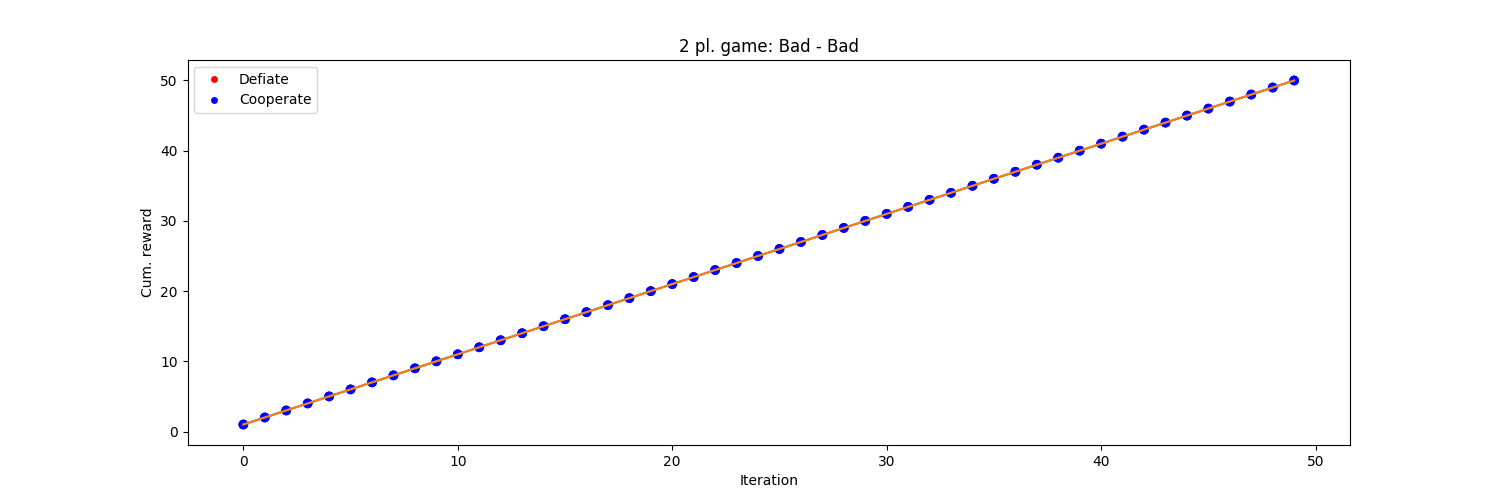
\includegraphics[width=1\columnwidth]{img_v1/idp2p-rewards-Bad-Bad.png}
    \caption{Bad guy vs bad guy}
    \label{fig:badvsbad}
\end{figure}

\begin{figure}
    \centering
    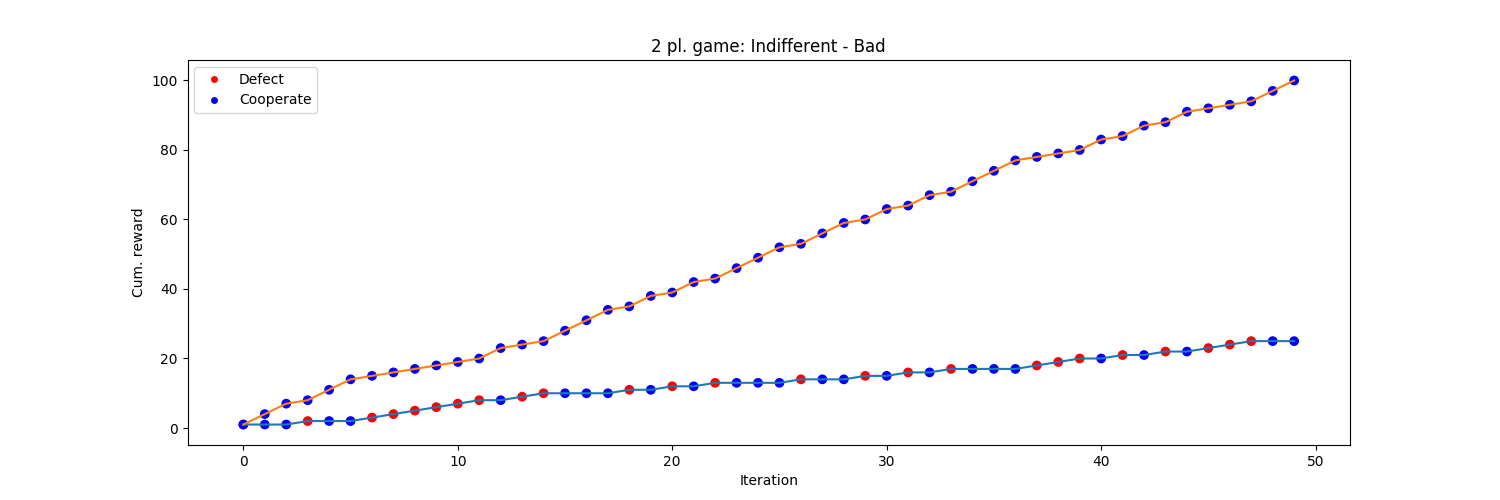
\includegraphics[width=1\columnwidth]{img_v1/idp2p-rewards-Indifferent-Bad.png}
    \caption{Bad guy vs Indifferent}
    \label{fig:badvsindiff}
\end{figure}

\begin{figure}
    \centering
    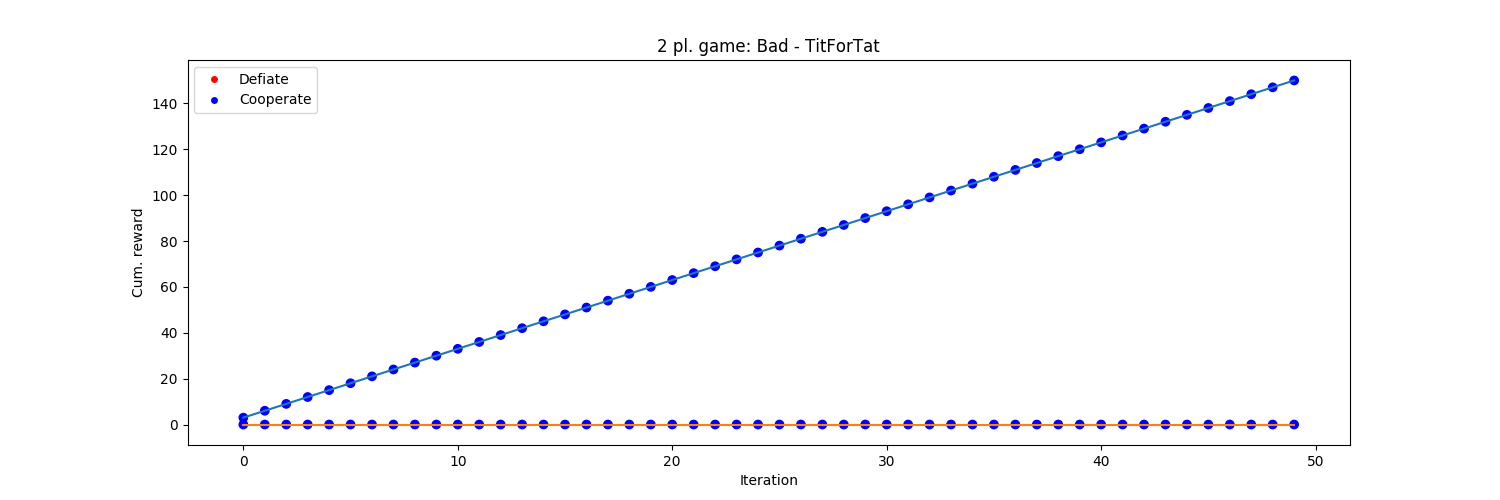
\includegraphics[width=1\columnwidth]{img_v1/idp2p-rewards-Bad-TitForTat.png}
    \caption{Bad guy vs TfT}
    \label{fig:badvstft}
\end{figure}

\begin{figure}
    \centering
    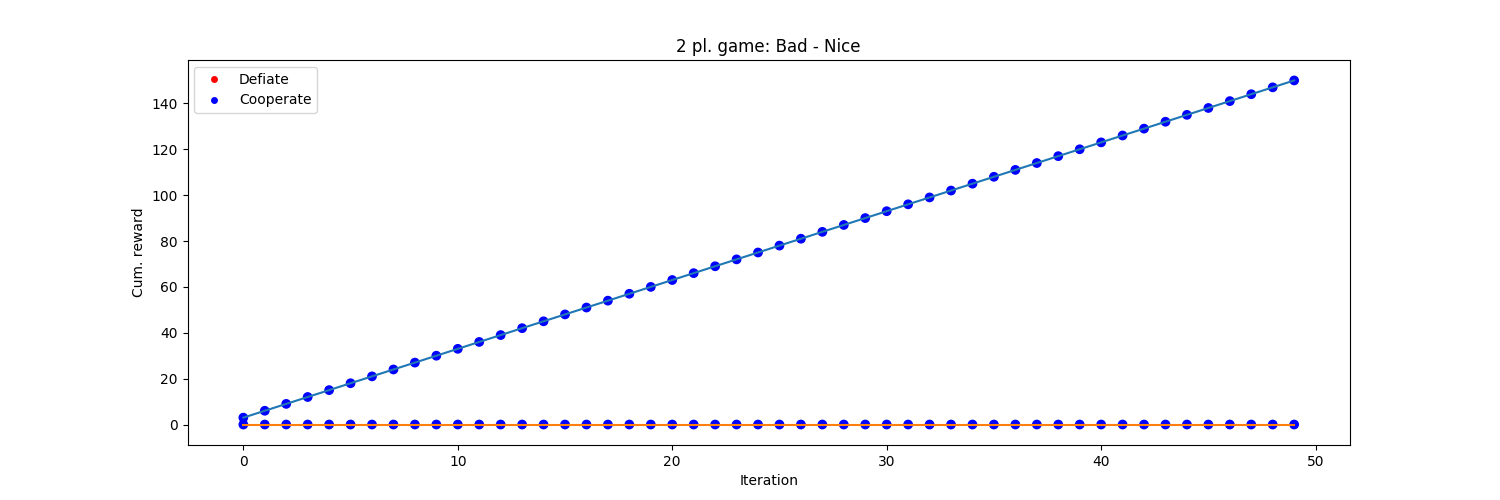
\includegraphics[width=1\columnwidth]{img_v1/idp2p-rewards-Bad-Nice.png}
    \caption{Bad guy vs Nice guy}
    \label{fig:badvsnice}
\end{figure}

%fix: because there is a space in the image!
\begin{figure}
    \centering
    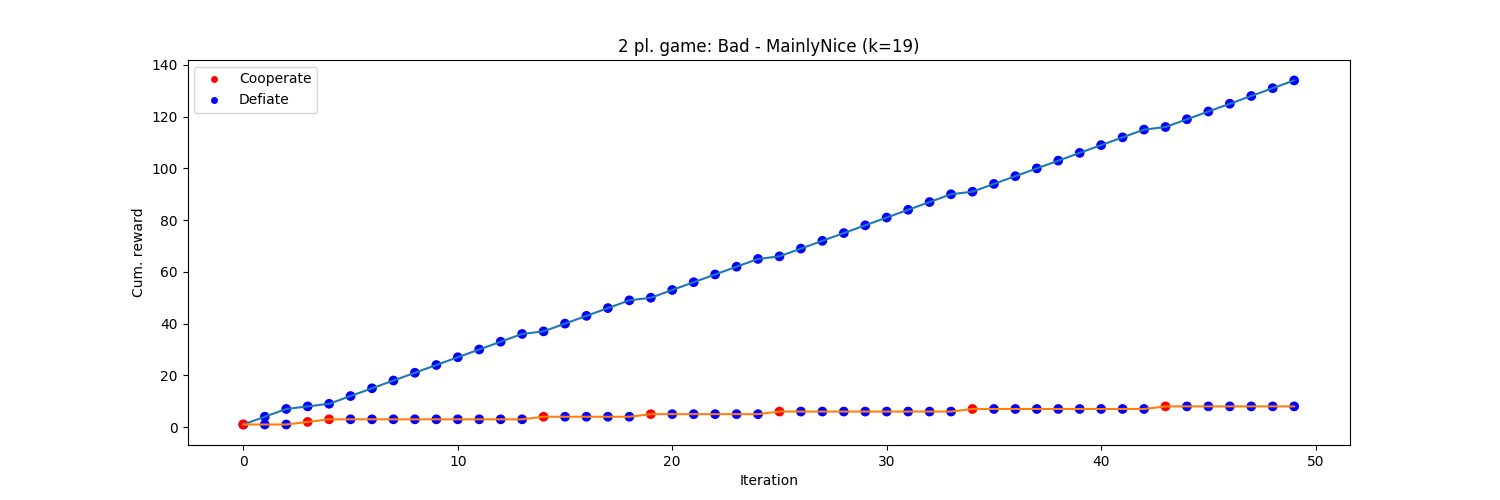
\includegraphics[width=1\columnwidth]{img_v1/idp2p-rewards-Bad-MainlyNice (k=19).png}
    \caption{Bad guy vs Mainly nice guy}
    \label{fig:badvsmainlynice}
\end{figure}

%fix: because there is a space in the image!
\begin{figure}
    \centering
    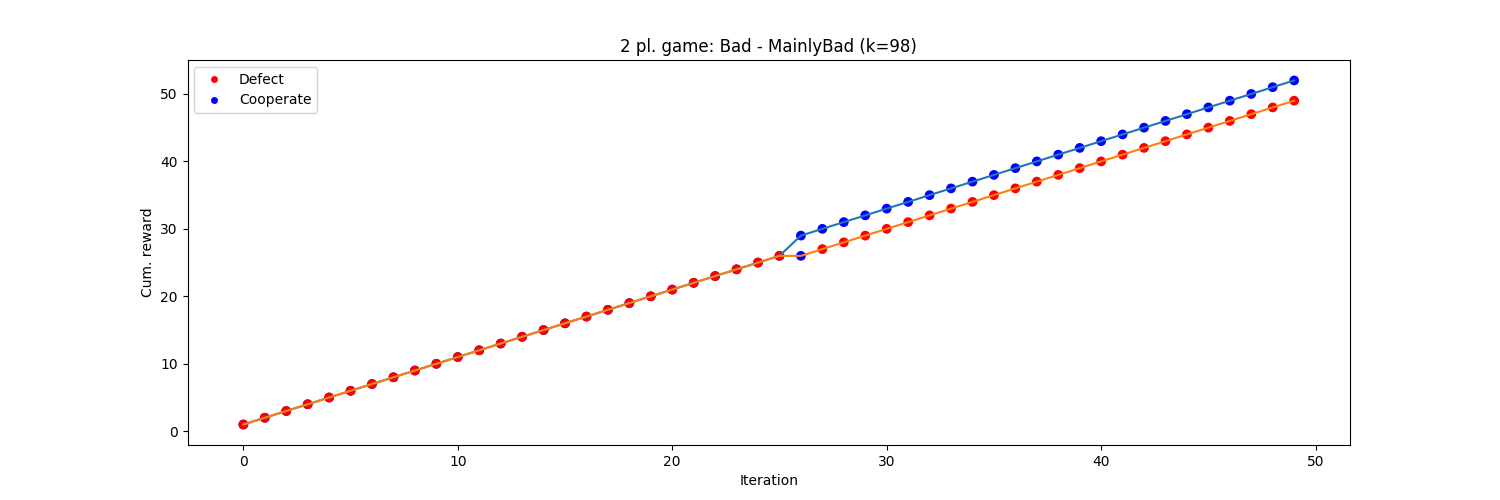
\includegraphics[width=1\columnwidth]{img_v1/idp2p-rewards-Bad-MainlyBad (k=98).png}
    \caption{Bad guy vs Mainly bad guy}
    \label{fig:badvsmainlybad}
\end{figure}

Infact, players might consider a different combination of strategies if they both want to get the highest reward possible: Indifferent-Indifferent, Indifferent-TfT, Nice-Nice or Nice-TfT, TfT-TfT as in \autoref{fig:indiffvsindiff}, \autoref{fig:tftvsindiff}, \autoref{fig:nicevsnice}, \autoref{fig:nicevstft}, \autoref{fig:tftvstft}.

\begin{figure}
    \centering
    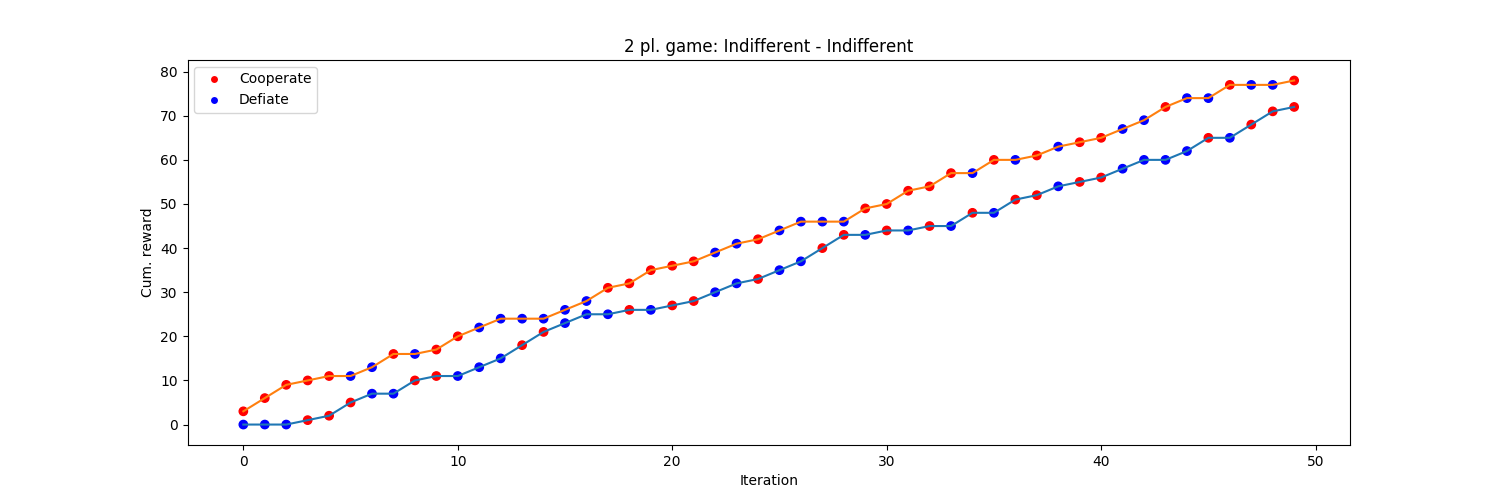
\includegraphics[width=1\columnwidth]{img_v1/idp2p-rewards-Indifferent-Indifferent.png}
    \caption{Indifferent guy vs Indifferent guy}
    \label{fig:indiffvsindiff}
\end{figure}

\begin{figure}
    \centering
    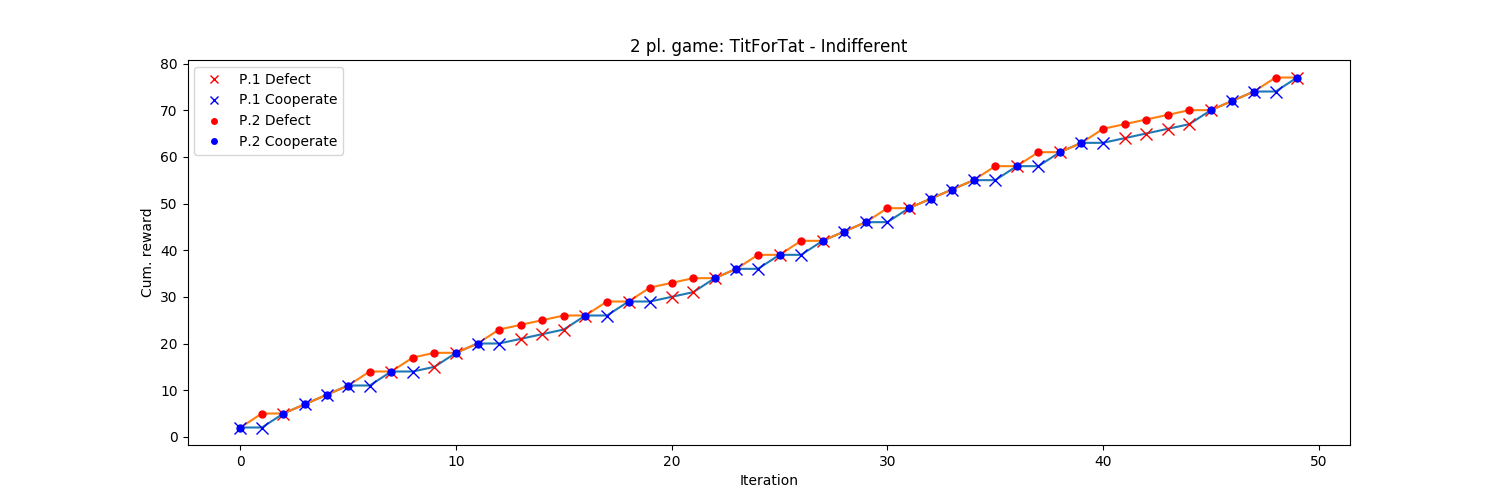
\includegraphics[width=1\columnwidth]{img_v1/idp2p-rewards-TitForTat-Indifferent.png}
    \caption{TfT vs Indifferent guy}
    \label{fig:tftvsindiff}
\end{figure}

\begin{figure}
    \centering
    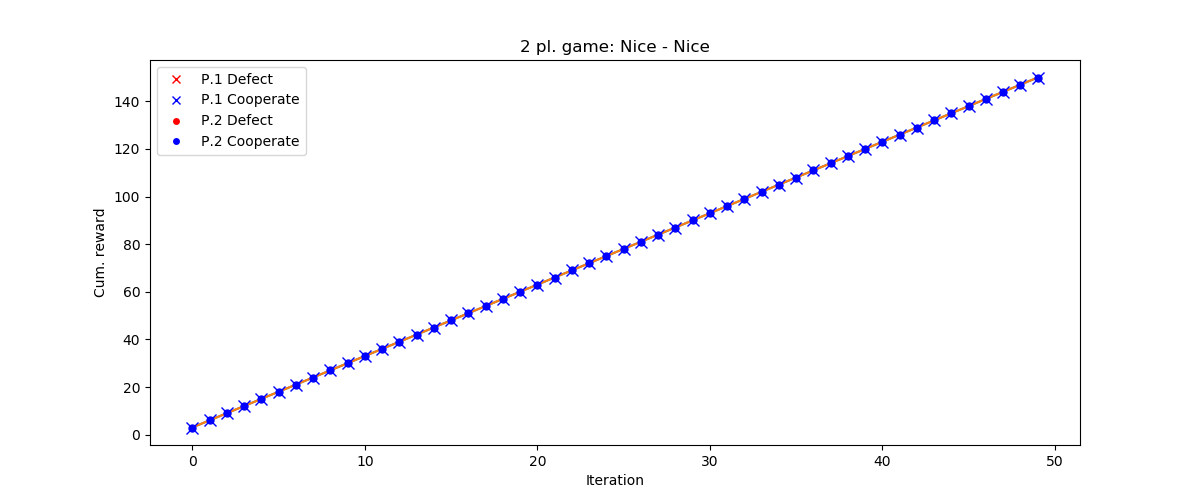
\includegraphics[width=1\columnwidth]{img_v1/idp2p-rewards-Nice-Nice.png}
    \caption{Nice guy vs Nice guy}
    \label{fig:nicevsnice}
\end{figure}

\begin{figure}
    \centering
    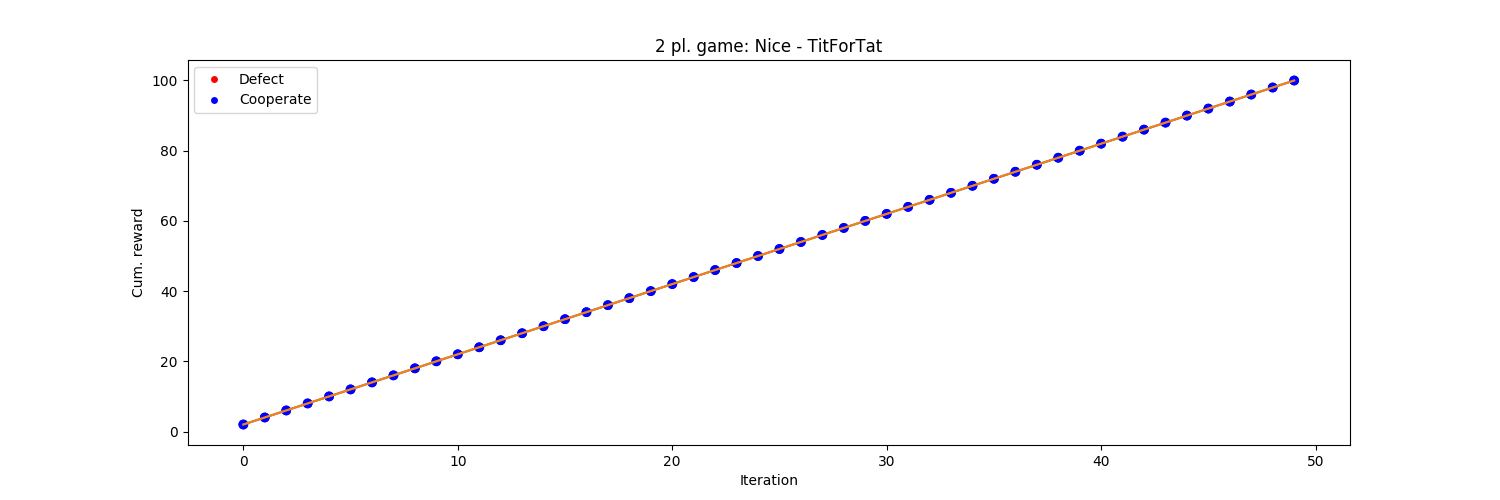
\includegraphics[width=1\columnwidth]{img_v1/idp2p-rewards-Nice-TitForTat.png}
    \caption{Nice guy vs TfT}
    \label{fig:nicevstft}
\end{figure}

\begin{figure}
    \centering
    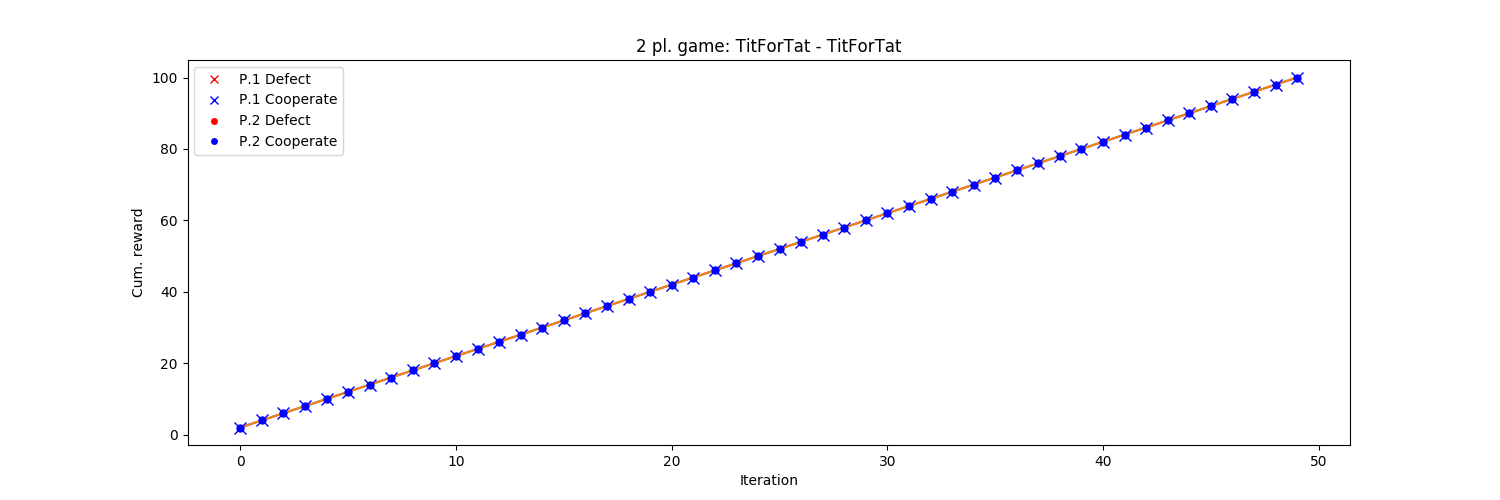
\includegraphics[width=1\columnwidth]{img_v1/idp2p-rewards-TitForTat-TitForTat.png}
    \caption{TfT vs TfT}
    \label{fig:tftvstft}
\end{figure}

The TfT strategy is interesting, because TfT leads almost to the same cumulative reward as the opponent. However it might be lower than one in some points, since it replicates the previous opponent's move and not the actual move. A player might choose this move if he wants almost the same reward as the opponent.

In conclusion if a player wants to be sure he wins over the other he/she should chose a \textit{Bad guy} strategy, if he/she wants to cooperate as much as possible he/she might choose \textit{TfT, Nice} or \textit{indifferent} hoping the opponent chooses the one of the strategies in this group.     

\newpage

\section{Multiple players IPD - Round-robin scheme}
In this section a multiple players IPD (MPIPD) is implemented. The round-robin scheme, used to match-up the opponents, consists in each player playing once against each other player in the torunament.
Each player chooses its fixed strategy at the beginning of the tournament and holds it throughout the course of the tournament.
As in IPD it is possible to set the number of iterations in each match (i.e $NUM\_ITER = 50$). In addition the number of players $n = 10$ determines the total number of matches played in the tournament, which in this case is $\dfrac{n \times (n-1)}{2} = 45$.

We propose a strategy, similar to \textit{Serie A} to assign points to each player after the outcome of the match is determined. A player gets 3 points if he/she wins, 1 point for a draw and 0 points for a loss. A player wins if he/she has a higher reward than the opponent's at the $50-th$ last iteration. He/She looses if the reward is lower and draws if it's the same as the opponent's.
The culumative points after each match are shown in \autoref{fig:mpipd}.
In \autoref{tab:ranking_df} the ranking of the torunament is determined. It can be evaluated that the three players using a \textit{Bad guy} strategy win the tournament.
The strategies can be sorted by most number of points as follows: \texit{Bad guy}, \textit{Mainly bad guy}, \textit{Indifferent}, \textit{Mainly Nice}, \textit{TitForTat} and \textit{Nice}.

\begin{figure}
    \centering
    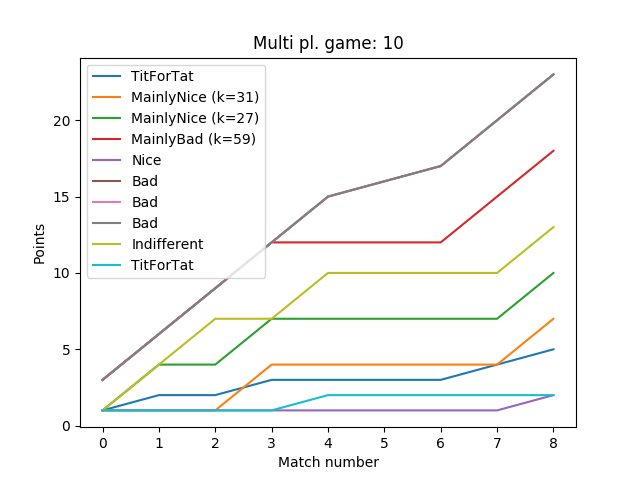
\includegraphics[width=1\columnwidth]{img_v1/idpmp-scores-10.png}
    \caption{Match number vs Points}
    \label{fig:mpipd}
\end{figure}

\begin{table}
    \centering
    \begin{tabular}{llrrrr}
    \toprule
    {} &             Player &  W &  D &  L &  points \\
    \midrule
    0 &                Bad &  7 &  2 &  0 &      23 \\
    0 &                Bad &  7 &  2 &  0 &      23 \\
    0 &                Bad &  7 &  2 &  0 &      23 \\
    0 &   MainlyBad (k=59) &  6 &  0 &  3 &      18 \\
    0 &        Indifferent &  4 &  1 &  4 &      13 \\
    0 &  MainlyNice (k=27) &  2 &  2 &  5 &       8 \\
    0 &  MainlyNice (k=31) &  2 &  1 &  6 &       7 \\
    0 &          TitForTat &  0 &  5 &  4 &       5 \\
    0 &          TitForTat &  0 &  3 &  6 &       3 \\
    0 &               Nice &  0 &  2 &  7 &       2 \\
    \bottomrule
    \end{tabular}
    
    \caption{Ranking table.}
    \label{tab:ranking_df}
\end{table}

The outcome of each match of the tournament can be seen in \autoref{tab:match_df}.
\begin{table}[]
    \centering
    \begin{tabular}{lllllrr}
    \toprule
    {} &                 p1 &                 p2 & p1-result & p2-result &  p1-score &  p2-score \\
    \midrule
    0 &          TitForTat &  MainlyNice (k=27) &         d &         d &        84 &        84 \\
    0 &          TitForTat &   MainlyBad (k=59) &         l &         w &        72 &        75 \\
    0 &          TitForTat &               Nice &         d &         d &       100 &       100 \\
    0 &          TitForTat &                Bad &         l &         w &        49 &        52 \\
    0 &          TitForTat &                Bad &         l &         w &        49 &        52 \\
    0 &          TitForTat &                Bad &         l &         w &        49 &        52 \\
    0 &          TitForTat &        Indifferent &         d &         d &        71 &        71 \\
    0 &          TitForTat &          TitForTat &         d &         d &       100 &       100 \\
    0 &  MainlyNice (k=31) &   MainlyBad (k=59) &         l &         w &        44 &       107 \\
    0 &  MainlyNice (k=31) &               Nice &         w &         l &       115 &        70 \\
    0 &  MainlyNice (k=31) &                Bad &         l &         w &        14 &       122 \\
    0 &  MainlyNice (k=31) &                Bad &         l &         w &        16 &       118 \\
    0 &  MainlyNice (k=31) &                Bad &         l &         w &        20 &       110 \\
    0 &  MainlyNice (k=31) &        Indifferent &         l &         w &        70 &        94 \\
    0 &  MainlyNice (k=31) &          TitForTat &         w &         l &        87 &        84 \\
    0 &  MainlyNice (k=27) &               Nice &         w &         l &       114 &        72 \\
    0 &  MainlyNice (k=27) &                Bad &         l &         w &        13 &       124 \\
    0 &  MainlyNice (k=27) &                Bad &         l &         w &        12 &       126 \\
    0 &  MainlyNice (k=27) &                Bad &         l &         w &        11 &       128 \\
    0 &  MainlyNice (k=27) &        Indifferent &         l &         w &        72 &        87 \\
    0 &  MainlyNice (k=27) &          TitForTat &         d &         d &        90 &        90 \\
    0 &   MainlyBad (k=59) &                Bad &         l &         w &        35 &        80 \\
    0 &   MainlyBad (k=59) &                Bad &         l &         w &        29 &        92 \\
    0 &   MainlyBad (k=59) &                Bad &         l &         w &        28 &        94 \\
    0 &   MainlyBad (k=59) &        Indifferent &         w &         l &        78 &        66 \\
    0 &   MainlyBad (k=59) &          TitForTat &         w &         l &        71 &        68 \\
    0 &               Nice &                Bad &         l &         w &         0 &       150 \\
    0 &               Nice &                Bad &         l &         w &         0 &       150 \\
    0 &               Nice &        Indifferent &         l &         w &        48 &       126 \\
    0 &               Nice &          TitForTat &         d &         d &       100 &       100 \\
    0 &                Bad &                Bad &         d &         d &        50 &        50 \\
    0 &                Bad &        Indifferent &         w &         l &       102 &        24 \\
    0 &                Bad &          TitForTat &         w &         l &        52 &        49 \\
    0 &                Bad &        Indifferent &         w &         l &       114 &        18 \\
    0 &                Bad &          TitForTat &         w &         l &        52 &        49 \\
    0 &                Bad &          TitForTat &         w &         l &        52 &        49 \\
    \bottomrule
    \end{tabular}
    \caption{Outcome of each match.}
    \label{tab:match_df}
\end{table}

\newpage
\section{Repeated multiple players IPD - Round-robin scheme}
In this section the MPIPD round-robin scheme tournament, is iterated: \textit{Repeated multiple players IPD (rMPIPD}.
At each tournament repetition, the population is increased adding players with strategies that depend on the results that strategies achieved in the previous iteration. 
%In our case the population is increasing by one individual that uses the strategy of the previous tournament's winner.
% todo: complete text based on teacher's answer

\begin{figure}
    \centering
    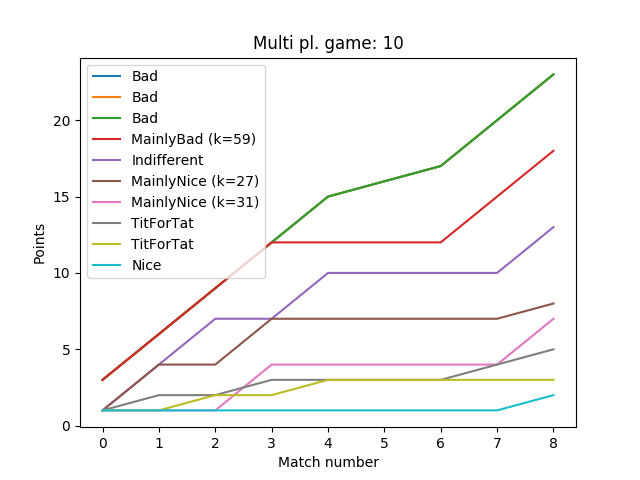
\includegraphics[width=1\columnwidth]{img_v1/ridpmp-scores-10-r0.png}
    \caption{Match number vs Points at repetition: 1.}
    \label{fig:rmpipd1}
\end{figure}

\begin{figure}
    \centering
    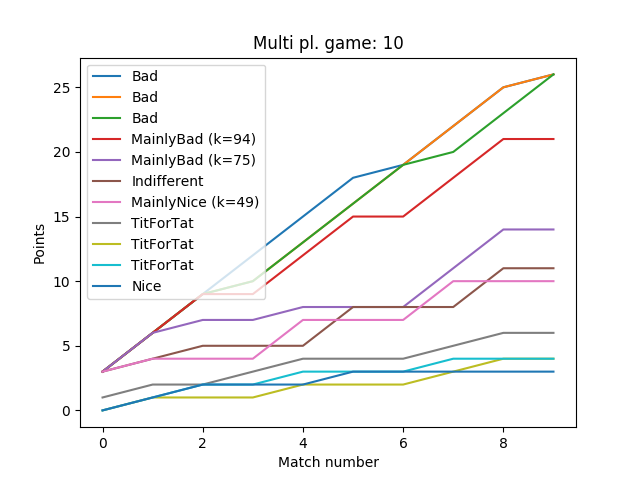
\includegraphics[width=1\columnwidth]{img_v1/ridpmp-scores-10-r1.png}
    \caption{Match number vs Points at repetition: 2.}
    \label{fig:rmpipd2}
\end{figure}

\begin{figure}
    \centering
    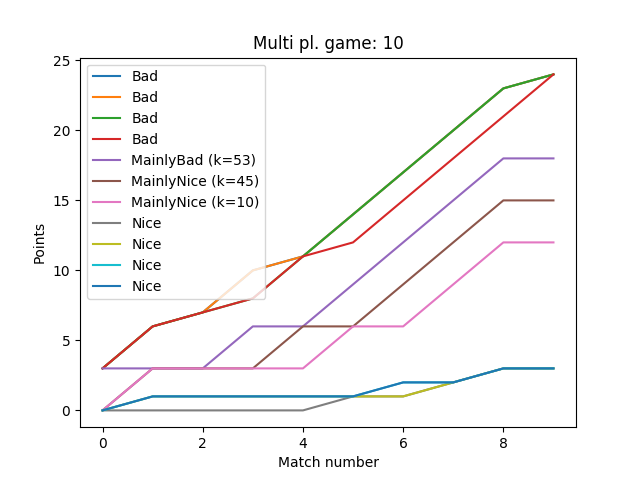
\includegraphics[width=1\columnwidth]{img_v1/ridpmp-scores-10-r2.png}
    \caption{Match number vs Points at repetition: 3.}
    \label{fig:rmpipd3}
\end{figure}

\begin{figure}
    \centering
    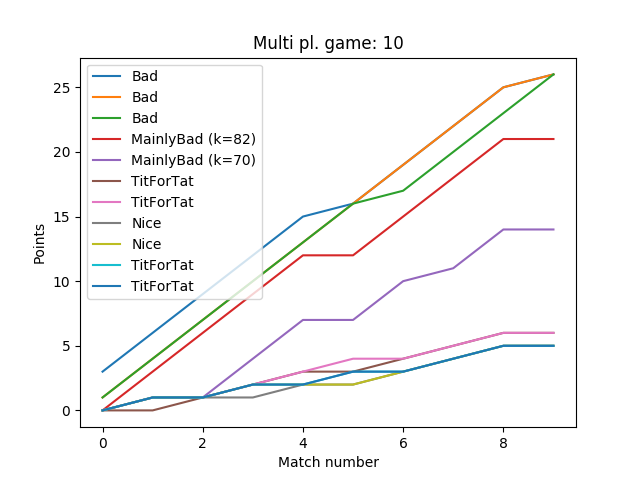
\includegraphics[width=1\columnwidth]{img_v1/ridpmp-scores-10-r3.png}
    \caption{Match number vs Points at repetition: 4.}
    \label{fig:rmpipd4}
\end{figure}

\begin{figure}
    \centering
    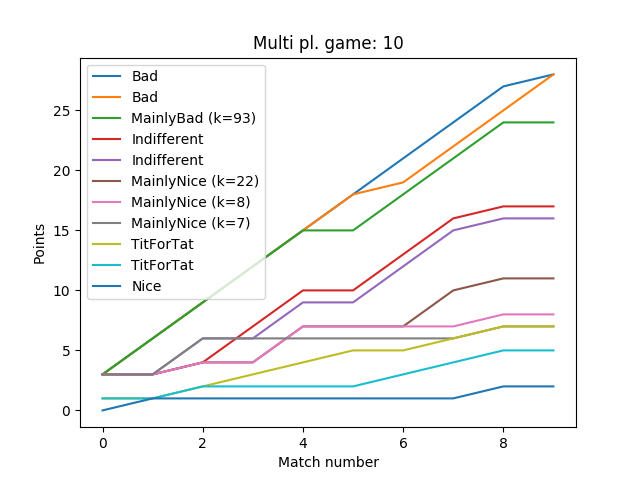
\includegraphics[width=1\columnwidth]{img_v1/ridpmp-scores-10-r4.png}
    \caption{Match number vs Points at repetition: 5.}
    \label{fig:rmpipd5}
\end{figure}

\newpage
\section{Chainging rMPIPD - Round-Robin scheme}
In this section a rMPIPD where strategies are allowed to mutate is implemented. The gene, a parameter, encodes the attitude of an individual to cooperate. This gene mutates randomly to choose a different strategy at each iteration. The phenotype, which is the strategy, corresponding to that gene competes in the MPIPD such that the best-fitted, which is the winner of the tournament, is determined.

The goal of this task is to simulate the effect of genetic mutations and the effect of natura selection.

In \autoref{fig:cmpipd1} all the players change strategy at each iteration when competing against other players. \textit{Player 7} wins the tournament and the ranking is shown in \autoref{tab:cmpipd1}.

% todo: complete based on teacher's answer

\begin{figure}
    \centering
    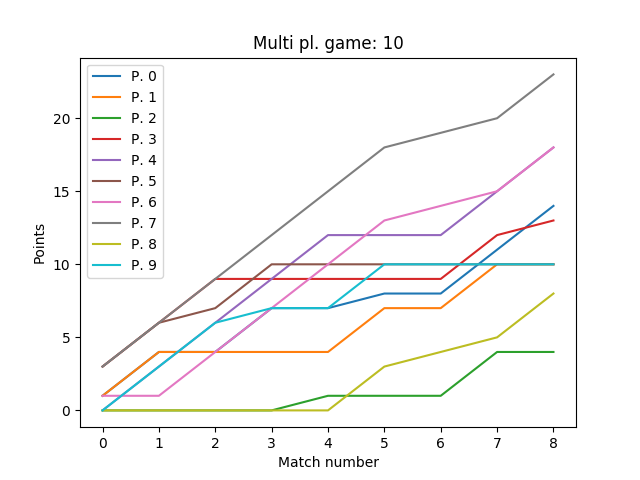
\includegraphics[width=1\columnwidth]{img_v1/cidpmp-scores-10.png}
    \caption{Match number vs Points at repetition: 1.}
    \label{fig:cmpipd1}
\end{figure}

\begin{table}[]
    \centering
    \begin{tabular}{lrrrrr}
    \toprule
    {} &  Player &  W &  D &  L &  points \\
    \midrule
    0 &       7 &  7 &  2 &  0 &      23 \\
    0 &       4 &  6 &  0 &  3 &      18 \\
    0 &       6 &  5 &  3 &  1 &      18 \\
    0 &       0 &  4 &  2 &  3 &      14 \\
    0 &       3 &  4 &  1 &  4 &      13 \\
    0 &       1 &  3 &  1 &  5 &      10 \\
    0 &       5 &  3 &  1 &  5 &      10 \\
    0 &       9 &  3 &  1 &  5 &      10 \\
    0 &       8 &  2 &  2 &  5 &       8 \\
    0 &       2 &  1 &  1 &  7 &       4 \\
    \bottomrule
    \end{tabular}
    \caption{Ranking table at repetition: 1.}
    \label{tab:cmpipd1}
\end{table}

%\bibliographystyle{IEEEtran}
%\bibliography{report.bib}
\end{document}
